\section{Analyze attack trends}\label{analyze-attack-trends}

\begingroup\fontsize{9}{11}\selectfont

\begin{longtable}[t]{llllrrrrrr}
\caption{\label{tab:arbitrary_trend_table}We run a logistic model regressing success against perturb-target distance and perturb box length, both relative to image width or height, in the deliberate attack experiment. Longer perturb box length or shorter perturb-target distance cause success rates to significantly increase for all model and attack combinations, except for perturb box length in untargeted attack on Cascade R-CNN. The interaction terms, even when significant, are negligibly close to 0. Table headers are explained in Appendix \ref{app:tab_hdr}.}\\
\toprule
\multicolumn{2}{c}{Group} & \multicolumn{8}{c}{Regression} \\
\cmidrule(l{3pt}r{3pt}){1-2} \cmidrule(l{3pt}r{3pt}){3-10}
 & Attack & term & sig & estimate & std.error & statistic & p.value & conf.low & conf.high\\
\midrule
\addlinespace[0.3em]
\multicolumn{10}{l}{\textbf{YOLOv3}}\\
\hspace{1em} & Vanishing & distance & * & -6.047 & 1.227 & -4.928 & 0.000 & -8.472 & -3.660\\
\cmidrule{3-10}\nopagebreak
\hspace{1em} &  & length & * & 8.243 & 0.530 & 15.558 & 0.000 & 7.227 & 9.305\\
\cmidrule{3-10}\nopagebreak
\hspace{1em} &  & distance * length & * & -18.211 & 3.543 & -5.140 & 0.000 & -25.189 & -11.292\\
\cmidrule{2-10}\nopagebreak
\hspace{1em} & Mislabeling & distance & * & -7.151 & 1.231 & -5.810 & 0.000 & -9.588 & -4.761\\
\cmidrule{3-10}\nopagebreak
\hspace{1em} &  & length & * & 5.888 & 0.395 & 14.922 & 0.000 & 5.126 & 6.674\\
\cmidrule{3-10}\nopagebreak
\hspace{1em} &  & distance * length &  & -3.239 & 3.100 & -1.045 & 0.296 & -9.296 & 2.862\\
\cmidrule{2-10}\nopagebreak
\hspace{1em} & Untargeted & distance & * & -9.320 & 1.515 & -6.153 & 0.000 & -12.343 & -6.401\\
\cmidrule{3-10}\nopagebreak
\hspace{1em} &  & length & * & 2.063 & 0.285 & 7.245 & 0.000 & 1.508 & 2.624\\
\cmidrule{3-10}\nopagebreak
\hspace{1em} &  & distance * length &  & 4.340 & 2.943 & 1.475 & 0.140 & -1.392 & 10.150\\
\cmidrule{1-10}\pagebreak[0]
\addlinespace[0.3em]
\multicolumn{10}{l}{\textbf{SSD}}\\
\hspace{1em} & Vanishing & distance & * & -10.417 & 1.552 & -6.711 & 0.000 & -13.513 & -7.424\\
\cmidrule{3-10}\nopagebreak
\hspace{1em} &  & length & * & 4.737 & 0.318 & 14.882 & 0.000 & 4.120 & 5.368\\
\cmidrule{3-10}\nopagebreak
\hspace{1em} &  & distance * length &  & -3.353 & 3.072 & -1.091 & 0.275 & -9.345 & 2.705\\
\cmidrule{2-10}\nopagebreak
\hspace{1em} & Mislabeling & distance & * & -7.996 & 1.697 & -4.712 & 0.000 & -11.385 & -4.729\\
\cmidrule{3-10}\nopagebreak
\hspace{1em} &  & length & * & 6.065 & 0.345 & 17.570 & 0.000 & 5.397 & 6.750\\
\cmidrule{3-10}\nopagebreak
\hspace{1em} &  & distance * length & * & -12.651 & 3.354 & -3.772 & 0.000 & -19.201 & -6.047\\
\cmidrule{2-10}\nopagebreak
\hspace{1em} & Untargeted & distance & * & -9.777 & 1.868 & -5.233 & 0.000 & -13.530 & -6.201\\
\cmidrule{3-10}\nopagebreak
\hspace{1em} &  & length & * & 3.798 & 0.314 & 12.094 & 0.000 & 3.188 & 4.419\\
\cmidrule{3-10}\nopagebreak
\hspace{1em} &  & distance * length & * & -7.443 & 3.635 & -2.048 & 0.041 & -14.527 & -0.268\\
\cmidrule{1-10}\pagebreak[0]
\addlinespace[0.3em]
\multicolumn{10}{l}{\textbf{RetinaNet}}\\
\hspace{1em} & Vanishing & distance & * & -23.008 & 3.077 & -7.477 & 0.000 & -29.253 & -17.194\\
\cmidrule{3-10}\nopagebreak
\hspace{1em} &  & length & * & 2.583 & 0.345 & 7.491 & 0.000 & 1.912 & 3.264\\
\cmidrule{3-10}\nopagebreak
\hspace{1em} &  & distance * length &  & -10.769 & 6.353 & -1.695 & 0.090 & -23.153 & 1.757\\
\cmidrule{2-10}\nopagebreak
\hspace{1em} & Mislabeling & distance & * & -22.522 & 4.237 & -5.316 & 0.000 & -31.273 & -14.667\\
\cmidrule{3-10}\nopagebreak
\hspace{1em} &  & length & * & 1.261 & 0.419 & 3.007 & 0.003 & 0.443 & 2.087\\
\cmidrule{3-10}\nopagebreak
\hspace{1em} &  & distance * length &  & 1.459 & 8.334 & 0.175 & 0.861 & -14.680 & 18.011\\
\cmidrule{2-10}\nopagebreak
\hspace{1em} & Untargeted & distance & * & -23.500 & 2.437 & -9.643 & 0.000 & -28.382 & -18.828\\
\cmidrule{3-10}\nopagebreak
\hspace{1em} &  & length & * & 2.528 & 0.334 & 7.571 & 0.000 & 1.880 & 3.189\\
\cmidrule{3-10}\nopagebreak
\hspace{1em} &  & distance * length & * & 37.697 & 4.191 & 8.994 & 0.000 & 29.615 & 46.048\\
\cmidrule{1-10}\pagebreak[0]
\addlinespace[0.3em]
\multicolumn{10}{l}{\textbf{Faster R-CNN}}\\
\hspace{1em} & Vanishing & distance & * & -31.756 & 3.996 & -7.947 & 0.000 & -39.875 & -24.217\\
\cmidrule{3-10}\nopagebreak
\hspace{1em} &  & length & * & 2.075 & 0.360 & 5.770 & 0.000 & 1.375 & 2.785\\
\cmidrule{3-10}\nopagebreak
\hspace{1em} &  & distance * length &  & -0.099 & 7.820 & -0.013 & 0.990 & -15.305 & 15.352\\
\cmidrule{2-10}\nopagebreak
\hspace{1em} & Mislabeling & distance & * & -28.038 & 4.331 & -6.474 & 0.000 & -36.927 & -19.955\\
\cmidrule{3-10}\nopagebreak
\hspace{1em} &  & length & * & 0.955 & 0.395 & 2.419 & 0.016 & 0.185 & 1.734\\
\cmidrule{3-10}\nopagebreak
\hspace{1em} &  & distance * length &  & 10.044 & 8.211 & 1.223 & 0.221 & -5.864 & 26.342\\
\cmidrule{2-10}\nopagebreak
\hspace{1em} & Untargeted & distance & * & -29.741 & 2.761 & -10.770 & 0.000 & -35.304 & -24.477\\
\cmidrule{3-10}\nopagebreak
\hspace{1em} &  & length & * & 1.494 & 0.312 & 4.783 & 0.000 & 0.886 & 2.111\\
\cmidrule{3-10}\nopagebreak
\hspace{1em} &  & distance * length & * & 36.707 & 4.548 & 8.071 & 0.000 & 27.946 & 45.780\\
\cmidrule{1-10}\pagebreak[0]
\addlinespace[0.3em]
\multicolumn{10}{l}{\textbf{Cascade R-CNN}}\\
\hspace{1em} & Vanishing & distance & * & -33.193 & 4.280 & -7.755 & 0.000 & -41.863 & -25.092\\
\cmidrule{3-10}\nopagebreak
\hspace{1em} &  & length & * & 3.929 & 0.405 & 9.706 & 0.000 & 3.145 & 4.732\\
\cmidrule{3-10}\nopagebreak
\hspace{1em} &  & distance * length & * & -22.519 & 8.925 & -2.523 & 0.012 & -39.964 & -4.967\\
\cmidrule{2-10}\nopagebreak
\hspace{1em} & Mislabeling & distance & * & -34.815 & 5.234 & -6.652 & 0.000 & -45.560 & -25.047\\
\cmidrule{3-10}\nopagebreak
\hspace{1em} &  & length & * & 1.853 & 0.395 & 4.698 & 0.000 & 1.085 & 2.632\\
\cmidrule{3-10}\nopagebreak
\hspace{1em} &  & distance * length &  & -2.173 & 10.288 & -0.211 & 0.833 & -22.101 & 18.246\\
\cmidrule{2-10}\nopagebreak
\hspace{1em} & Untargeted & distance & * & -45.652 & 4.120 & -11.080 & 0.000 & -53.998 & -37.841\\
\cmidrule{3-10}\nopagebreak
\hspace{1em} &  & length & * & 0.675 & 0.327 & 2.061 & 0.039 & 0.036 & 1.320\\
\cmidrule{3-10}\nopagebreak
\hspace{1em} &  & distance * length & * & 47.723 & 6.636 & 7.191 & 0.000 & 34.958 & 60.993\\
\bottomrule
\end{longtable}
\endgroup{}

\begin{figure}[tb]

{\centering 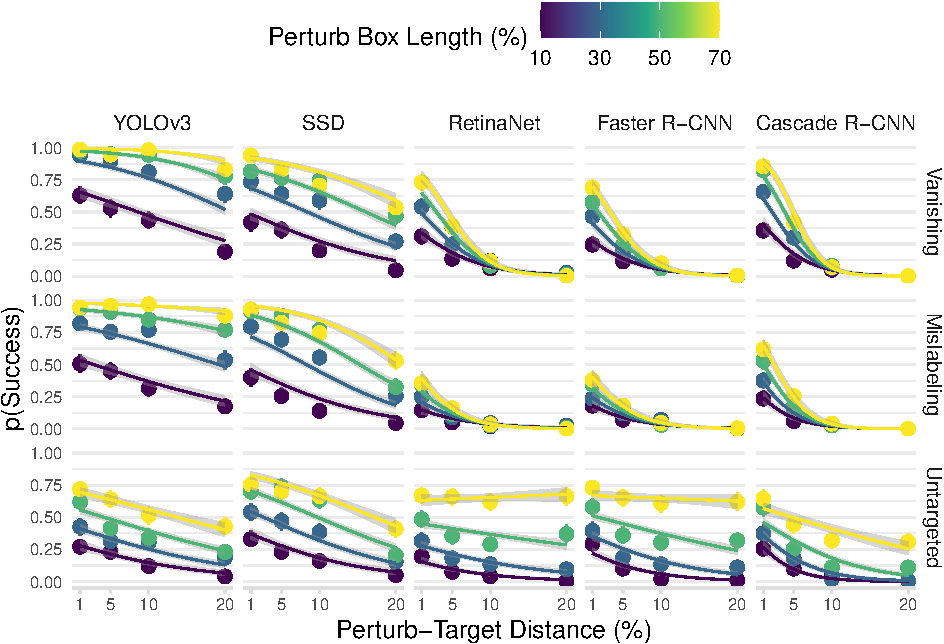
\includegraphics[width=1\linewidth]{imgs/arbitrary_trend_graph-1} 

}

\caption{Perturbing an arbitrary region obfuscates intent with increased success for all models and attacks even with 0.05 max-norm:  We implement intent obfuscating attack by perturbing an arbitrary non-overlapping square region to disrupt a randomly selected target object at various lengths and distances. The binned summaries and regression trendlines graph success proportion against perturb-target distance and perturb box length, both relative to image width or height, in the deliberate attack experiment. Errors are 95\% confidence intervals and every point aggregates success over 200 images. The deliberate attack multiplies success as compared to the randomized attack (Figure \ref{fig:success_trend_graph}), especially at close perturb-target distance and large perturb box length. Full details are given in Section \ref{sec:del_arb}.}\label{fig:arbitrary_trend_graph}
\end{figure}

\begingroup\fontsize{9}{11}\selectfont

\begin{longtable}[t]{llllrrrrrr}
\caption{\label{tab:rand_arb_compare_table}We combined the data in the randomized and deliberate attack experiments to run a logistic model regressing success against object (versus non-object), with perturb-target distance and perturb box size as covariates, both relative to image width or height. The ``object'' term codes object as 1 and non-object as 0. Perturbing an object (in the randomized attack) rather than a non-object (in the deliberate attack) significantly decreases success rates for all model and attack combinations, after controlling for perturb sizes and perturb-target distances. Table headers are explained in Appendix \ref{app:tab_hdr}.}\\
\toprule
\multicolumn{2}{c}{Group} & \multicolumn{8}{c}{Regression} \\
\cmidrule(l{3pt}r{3pt}){1-2} \cmidrule(l{3pt}r{3pt}){3-10}
 & Attack & term & sig & estimate & std.error & statistic & p.value & conf.low & conf.high\\
\midrule
\addlinespace[0.3em]
\multicolumn{10}{l}{\textbf{YOLOv3}}\\
\hspace{1em} & Vanishing & object &  & -0.126 & 0.069 & -1.829 & 0.067 & -0.260 & 0.009\\
\cmidrule{3-10}\nopagebreak
\hspace{1em} &  & distance & * & -9.446 & 0.482 & -19.592 & 0.000 & -10.405 & -8.515\\
\cmidrule{3-10}\nopagebreak
\hspace{1em} &  & size & * & 16.353 & 0.900 & 18.179 & 0.000 & 14.634 & 18.161\\
\cmidrule{3-10}\nopagebreak
\hspace{1em} &  & distance * size & * & -43.789 & 4.938 & -8.867 & 0.000 & -53.633 & -34.267\\
\cmidrule{2-10}\nopagebreak
\hspace{1em} & Mislabeling & object & * & -0.254 & 0.064 & -3.985 & 0.000 & -0.379 & -0.129\\
\cmidrule{3-10}\nopagebreak
\hspace{1em} &  & distance & * & -8.051 & 0.428 & -18.833 & 0.000 & -8.902 & -7.226\\
\cmidrule{3-10}\nopagebreak
\hspace{1em} &  & size & * & 7.939 & 0.471 & 16.845 & 0.000 & 7.034 & 8.882\\
\cmidrule{3-10}\nopagebreak
\hspace{1em} &  & distance * size & * & -7.100 & 3.004 & -2.364 & 0.018 & -13.029 & -1.249\\
\cmidrule{2-10}\nopagebreak
\hspace{1em} & Untargeted & object & * & -0.533 & 0.078 & -6.807 & 0.000 & -0.687 & -0.380\\
\cmidrule{3-10}\nopagebreak
\hspace{1em} &  & distance & * & -10.771 & 0.730 & -14.752 & 0.000 & -12.232 & -9.370\\
\cmidrule{3-10}\nopagebreak
\hspace{1em} &  & size & * & 2.091 & 0.286 & 7.317 & 0.000 & 1.532 & 2.653\\
\cmidrule{3-10}\nopagebreak
\hspace{1em} &  & distance * size & * & 12.506 & 2.646 & 4.726 & 0.000 & 7.335 & 17.711\\
\cmidrule{1-10}\pagebreak[0]
\addlinespace[0.3em]
\multicolumn{10}{l}{\textbf{SSD}}\\
\hspace{1em} & Vanishing & object & * & 1.143 & 0.069 & 16.606 & 0.000 & 1.009 & 1.278\\
\cmidrule{3-10}\nopagebreak
\hspace{1em} &  & distance & * & -13.732 & 0.574 & -23.911 & 0.000 & -14.878 & -12.627\\
\cmidrule{3-10}\nopagebreak
\hspace{1em} &  & size & * & 5.475 & 0.339 & 16.160 & 0.000 & 4.819 & 6.147\\
\cmidrule{3-10}\nopagebreak
\hspace{1em} &  & distance * size &  & 1.736 & 2.532 & 0.686 & 0.493 & -3.244 & 6.686\\
\cmidrule{2-10}\nopagebreak
\hspace{1em} & Mislabeling & object & * & 0.887 & 0.069 & 12.813 & 0.000 & 0.752 & 1.023\\
\cmidrule{3-10}\nopagebreak
\hspace{1em} &  & distance & * & -11.787 & 0.585 & -20.137 & 0.000 & -12.957 & -10.663\\
\cmidrule{3-10}\nopagebreak
\hspace{1em} &  & size & * & 6.622 & 0.346 & 19.126 & 0.000 & 5.952 & 7.309\\
\cmidrule{3-10}\nopagebreak
\hspace{1em} &  & distance * size & * & -10.236 & 2.674 & -3.829 & 0.000 & -15.506 & -5.022\\
\cmidrule{2-10}\nopagebreak
\hspace{1em} & Untargeted & object & * & 0.914 & 0.070 & 12.977 & 0.000 & 0.777 & 1.053\\
\cmidrule{3-10}\nopagebreak
\hspace{1em} &  & distance & * & -12.866 & 0.654 & -19.665 & 0.000 & -14.176 & -11.611\\
\cmidrule{3-10}\nopagebreak
\hspace{1em} &  & size & * & 3.596 & 0.288 & 12.503 & 0.000 & 3.036 & 4.164\\
\cmidrule{3-10}\nopagebreak
\hspace{1em} &  & distance * size &  & -0.763 & 2.732 & -0.279 & 0.780 & -6.149 & 4.566\\
\cmidrule{1-10}\pagebreak[0]
\addlinespace[0.3em]
\multicolumn{10}{l}{\textbf{RetinaNet}}\\
\hspace{1em} & Vanishing & object &  & -0.034 & 0.086 & -0.395 & 0.693 & -0.203 & 0.135\\
\cmidrule{3-10}\nopagebreak
\hspace{1em} &  & distance & * & -30.751 & 1.730 & -17.775 & 0.000 & -34.225 & -27.443\\
\cmidrule{3-10}\nopagebreak
\hspace{1em} &  & size & * & 2.620 & 0.343 & 7.634 & 0.000 & 1.953 & 3.299\\
\cmidrule{3-10}\nopagebreak
\hspace{1em} &  & distance * size &  & 9.753 & 5.793 & 1.684 & 0.092 & -1.711 & 21.010\\
\cmidrule{2-10}\nopagebreak
\hspace{1em} & Mislabeling & object &  & 0.037 & 0.116 & 0.322 & 0.747 & -0.191 & 0.264\\
\cmidrule{3-10}\nopagebreak
\hspace{1em} &  & distance & * & -33.503 & 2.676 & -12.518 & 0.000 & -38.938 & -28.446\\
\cmidrule{3-10}\nopagebreak
\hspace{1em} &  & size & * & 0.871 & 0.419 & 2.080 & 0.038 & 0.051 & 1.693\\
\cmidrule{3-10}\nopagebreak
\hspace{1em} &  & distance * size & * & 23.197 & 8.508 & 2.726 & 0.006 & 6.307 & 39.700\\
\cmidrule{2-10}\nopagebreak
\hspace{1em} & Untargeted & object &  & -0.043 & 0.081 & -0.522 & 0.601 & -0.202 & 0.117\\
\cmidrule{3-10}\nopagebreak
\hspace{1em} &  & distance & * & -13.217 & 0.915 & -14.441 & 0.000 & -15.053 & -11.466\\
\cmidrule{3-10}\nopagebreak
\hspace{1em} &  & size & * & 3.032 & 0.295 & 10.289 & 0.000 & 2.456 & 3.611\\
\cmidrule{3-10}\nopagebreak
\hspace{1em} &  & distance * size & * & 33.609 & 2.898 & 11.599 & 0.000 & 28.011 & 39.372\\
\cmidrule{1-10}\pagebreak[0]
\addlinespace[0.3em]
\multicolumn{10}{l}{\textbf{Faster R-CNN}}\\
\hspace{1em} & Vanishing & object & * & -0.478 & 0.105 & -4.529 & 0.000 & -0.686 & -0.272\\
\cmidrule{3-10}\nopagebreak
\hspace{1em} &  & distance & * & -31.827 & 2.118 & -15.029 & 0.000 & -36.100 & -27.798\\
\cmidrule{3-10}\nopagebreak
\hspace{1em} &  & size & * & 2.432 & 0.382 & 6.368 & 0.000 & 1.689 & 3.186\\
\cmidrule{3-10}\nopagebreak
\hspace{1em} &  & distance * size &  & -3.404 & 7.606 & -0.448 & 0.654 & -18.494 & 11.337\\
\cmidrule{2-10}\nopagebreak
\hspace{1em} & Mislabeling & object & * & -0.636 & 0.133 & -4.778 & 0.000 & -0.900 & -0.378\\
\cmidrule{3-10}\nopagebreak
\hspace{1em} &  & distance & * & -26.142 & 2.304 & -11.348 & 0.000 & -30.831 & -21.799\\
\cmidrule{3-10}\nopagebreak
\hspace{1em} &  & size & * & 0.908 & 0.419 & 2.168 & 0.030 & 0.086 & 1.730\\
\cmidrule{3-10}\nopagebreak
\hspace{1em} &  & distance * size &  & 8.990 & 7.894 & 1.139 & 0.255 & -6.721 & 24.259\\
\cmidrule{2-10}\nopagebreak
\hspace{1em} & Untargeted & object & * & 0.272 & 0.084 & 3.241 & 0.001 & 0.108 & 0.437\\
\cmidrule{3-10}\nopagebreak
\hspace{1em} &  & distance & * & -13.071 & 0.864 & -15.131 & 0.000 & -14.804 & -11.418\\
\cmidrule{3-10}\nopagebreak
\hspace{1em} &  & size & * & 2.907 & 0.302 & 9.640 & 0.000 & 2.318 & 3.500\\
\cmidrule{3-10}\nopagebreak
\hspace{1em} &  & distance * size & * & 25.656 & 2.800 & 9.164 & 0.000 & 20.216 & 31.193\\
\cmidrule{1-10}\pagebreak[0]
\addlinespace[0.3em]
\multicolumn{10}{l}{\textbf{Cascade R-CNN}}\\
\hspace{1em} & Vanishing & object & * & -0.437 & 0.099 & -4.409 & 0.000 & -0.632 & -0.243\\
\cmidrule{3-10}\nopagebreak
\hspace{1em} &  & distance & * & -32.264 & 2.078 & -15.526 & 0.000 & -36.452 & -28.306\\
\cmidrule{3-10}\nopagebreak
\hspace{1em} &  & size & * & 5.213 & 0.426 & 12.239 & 0.000 & 4.392 & 6.063\\
\cmidrule{3-10}\nopagebreak
\hspace{1em} &  & distance * size & * & -42.522 & 8.789 & -4.838 & 0.000 & -60.059 & -25.581\\
\cmidrule{2-10}\nopagebreak
\hspace{1em} & Mislabeling & object & * & -0.314 & 0.112 & -2.803 & 0.005 & -0.535 & -0.096\\
\cmidrule{3-10}\nopagebreak
\hspace{1em} &  & distance & * & -32.423 & 2.526 & -12.835 & 0.000 & -37.559 & -27.654\\
\cmidrule{3-10}\nopagebreak
\hspace{1em} &  & size & * & 2.189 & 0.381 & 5.738 & 0.000 & 1.443 & 2.939\\
\cmidrule{3-10}\nopagebreak
\hspace{1em} &  & distance * size &  & -12.586 & 9.615 & -1.309 & 0.191 & -31.740 & 5.972\\
\cmidrule{2-10}\nopagebreak
\hspace{1em} & Untargeted & object &  & -0.075 & 0.091 & -0.825 & 0.409 & -0.255 & 0.103\\
\cmidrule{3-10}\nopagebreak
\hspace{1em} &  & distance & * & -19.039 & 1.269 & -15.008 & 0.000 & -21.594 & -16.620\\
\cmidrule{3-10}\nopagebreak
\hspace{1em} &  & size & * & 2.105 & 0.308 & 6.837 & 0.000 & 1.503 & 2.711\\
\cmidrule{3-10}\nopagebreak
\hspace{1em} &  & distance * size & * & 19.565 & 3.768 & 5.192 & 0.000 & 12.194 & 26.975\\
\bottomrule
\end{longtable}
\endgroup{}
